\documentclass{article}
\usepackage[utf8]{inputenc}
\usepackage{hyperref}
\usepackage{graphicx}
\graphicspath{ {./} }

\title{Thunder C++}
\author{Alberto Carli & Aleardo Lodi}
\date{Settembre 2022}

\begin{document}

\maketitle

\section{Link progetto originale}

\href{http://thunder-project.org/}{
Sito web del progetto}


\section{Descrizione del progetto}
Il nostro progetto é una riscrittura di una sezione del codice di \href{https://github.com/thunder-project/thunder}{thunder} in C++17.
Il progetto originario é una collezione di librerie, suddivisa in piú pacchetti, per importare immagini o serie dati e poi analizzarle.
Scritto in python puó essere eseguito in locale o con il supporto di uno Spark cluster.
Thunder é suddiviso in un core package che definisce delle semplici funzioni di lettura e scrittura dei dati e da vari pacchetti (si veda \href{https://github.com/thunder-project/thunder-regression}{questo} o \href{https://github.com/thunder-project/thunder-registration}{questo}) di supporto.

Il progetto non é piú in attivamente sviluppato e supportato, per cui durante la fase di benchmark abbiamo trovato alcune funzioni che tornano errori.


\section{Il porting}
\subsection{Scelte implementative}
Il nostro porting della libreria comprende due componenti principali: il caricamento dei dati e l'applicazione di alcune operazioni classiche sui dati.
Per quanto concerne il caricamento dei dati in un oggetto generico della nostra libreria é possible tramite vari sistemi:
\begin{itemize}
  \item Passare al costruttore C-like array o altri sequence
  \item Caricare un'immagine di tipo png
  \item Caricare un'immagine di tipo tif
  \item Estrarre una serie numerica o serie da un file
\end{itemize}

Questi dati vengono poi salvati in un vector all'interno della relativa classe che si basa su ndarray. Le funzioni di elaborazione dei dati appartengono alla classe ndarray, mentre funzioni specifiche per caricare e manipolare i dati appropriatamente si trovano nelle classi series e images.
Delle funzioni aggiuntive sono state scelte la maggior parte presente nel pacchetto base di \href{https://github.com/thunder-project/thunder}{thunder}.
Quali ad esempio: count, max, min, filter, std, var...


\section{Program workflow}
Innanzi tutto è necessario caricare i dati in qualche maniera. Si possono utilizzare diverse funzioni a seconda della classe, appropriate al tipo di struttura dati che vogliamo modellare e alle sue caratteristiche.
Successivamente si possono eseguire diverse manipolazioni e applicare diverse funzioni ai dati.

\section{I/O esempi}

Come dati d'input é possibile caricare immagini, array o serie numeriche.
Per quanto riguarda le serie numeriche basta che il file sia composto da numeri separati da uno spazio.
Le immagini devono essere di due formati, tif o png, per essere caricate e poi elaborate.
La procedura è molto semplice (stile python): data un oggetto supportato

\section{Code statistics}
\subsection{Coverage}
Man mano che venivano implementati i metodi venivano scritti anche i relativi unit test con ```Catch2``` fino al raggiungimento di una line coverage soddisfacente.
La coverage viene rilevata con ```lcov```, che viene utilizzato nel target ```make coverage```
per ottenere line, function e branch coverage, stamparla a schermo e generare, nella cartella ```doc/coverage```, un report in html.

\begin{figure}[h]
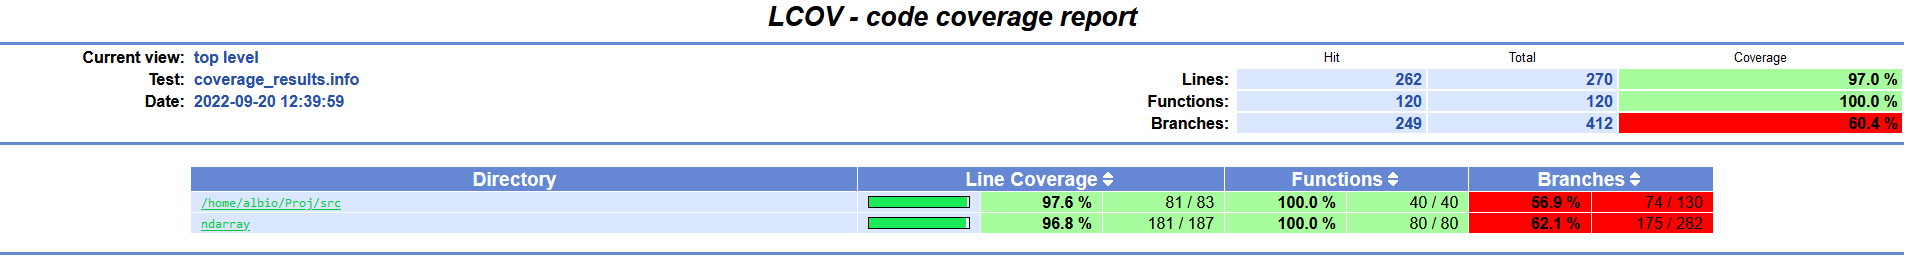
\includegraphics[width=\textwidth]{Coverage.png}
\end{figure}


\section{Static analysis}
Abbiamo eseguito diversi analizzatori statici e dinamici, quelli presentati all'interno del corso
\begin{itemize}
    \item Valgrind: All heap blocks were freed -- no leaks are possible
    \item Scan-build: No bugs found
\end{itemize}

\begin{figure}[h]
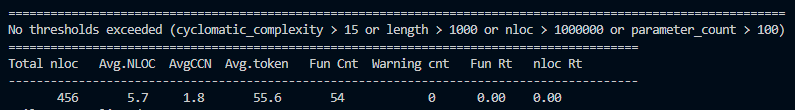
\includegraphics[width=\textwidth]{cyclomatic_complexity.png}
\end{figure}

Diversi possibili sanitizers sono stati aggiunti a tempo di compilazionee clang-tidy e clang-format sono stati lanciati su tutto il codice

\section{Testing}

É stata usata la libreria catch2 importata in third\_party/ per eseguire i test.
Per ogni componente principale sono stati creati dei file equivalenti per il testing, sia per testare il caricamento di file e immagini sia per tutte le funzioni create.



\section{Third party libraries}

Come librerie esterne é stato usato catch2 per testare il programma e CImg per poter leggere i file immagine e caricare in memoria immagini di vari formati.
É stata scelta questa libreria perché la piú semplice e che conteneva tutto quello che ci serviva per caricare le immagini.


\section{Performance C++ vs Python}

Come si puó vedere dai grafici sotto riportati le performance, con il flag di compilazione -O3, portano tutte C++ al primo posto come tempi di esecuzione.
Per quanto riguarda la lettura delle immagini direttamente da file non é stato possibile testare i file png.


\begin{figure}[h]
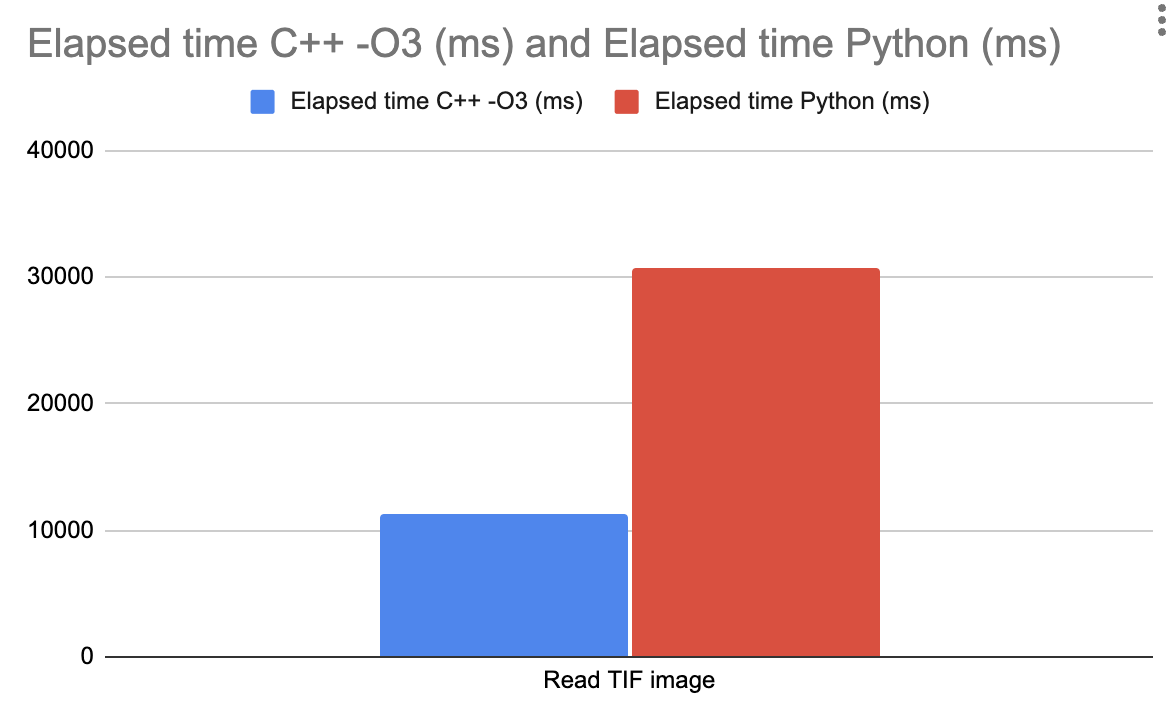
\includegraphics[width=\textwidth]{Performance 1.png}
\end{figure}
\begin{figure}[h]
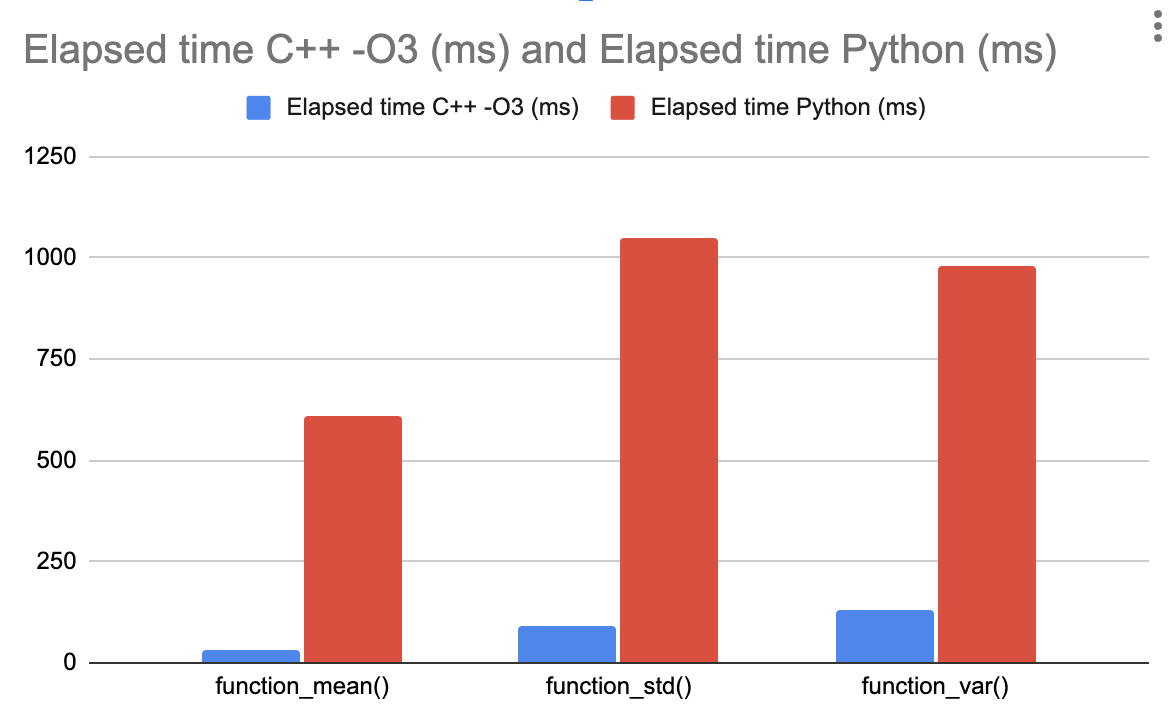
\includegraphics[width=\textwidth]{Performance 2.png}
\end{figure}


\end{document}
